% !TEX TS-program = XeLaTeX
%%%  یک نمونه پروژه/پایان‌نامه/رساله با استفاده از کلاس Tabriz_thesis، نسخه 1.1
%%%  وحید دامن‌افشان، دانشگاه صنعتی کرمانشاه،       http://www.damanafshan.ir
%%%  تالار گفتگوی پارسی‌لاتک،       http://forum.parsilatex.com
%%%   آپدیت شده در اسفند ۹۱

%-----------------------------------------------------------------------------------------------------
%        توجه داشته باشید برای دیدن خروجی کامل شامل نمایه و فهرست مطالب، ابتدا دو بار این فایل را
%        را اجرا کرده، سپس با استفاده از خط فرمان، به مسیر پوشه جاری رفته و دستور 
% xindy -L persian -C utf8 -M texindy -M page-ranges tabriz-thesis.idx
%        را در خط فرمان اجرا کنید. سپس دو بار دیگر، این فایل را اجرا کنید. 
%        اگر قصد نوشتن پروژه کارشناسی را دارید، در خط زیر به جای msc، کلمه bsc و اگر قصد نوشتن رساله دکتری
%        را دارید، کلمه phd را قرار دهید. کلیه تنظیمات لازم، به طور خودکار، اعمال می‌شود.
\documentclass[msc]{tabriz-thesis}
\csname@twosidetrue\endcsname
\usepackage{xepersian}
\settextfont[Scale=1.1]{XB Niloofar}
\defpersianfont\nastaliq[Scale=2]{IranNastaliq}
% چنانچه می‌خواهید اعداد در فرمول‌ها، انگلیسی باشد، خط زیر را غیرفعال کنید.
\setdigitfont[Scale=1.1]{Yas}
\begin{document}
\baselineskip=.75cm
\pagenumbering{harfi}
% در این فایل، عنوان پایان‌نامه، مشخصات خود، متن تقدیمی‌، ستایش، سپاس‌گزاری و چکیده پایان‌نامه را به فارسی، وارد کنید.
% توجه داشته باشید که جدول حاوی مشخصات پروژه/پایان‌نامه/رساله و همچنین، مشخصات داخل آن، به طور خودکار، درج می‌شود.
%%%%%%%%%%%%%%%%%%%%%%%%%%%%%%%%%%%%
% دانشگاه خود را وارد کنید
\university{تبریز}
% دانشکده، آموزشکده و یا پژوهشکده  خود را وارد کنید
\faculty{دانشکده علوم ریاضی}
% گروه آموزشی خود را وارد کنید
\department{گروه ریاضی محض}
% نام رشته تحصیلی خود را وارد کنید
\subject{ریاضی محض}
% گرایش خود را وارد کنید
\field{آنالیز ریاضی}
% عنوان پایان‌نامه را وارد کنید
\title{نوشتن پروژه، پایان‌نامه و رساله با استفاده از کلاس 
\lr{\textsf{tabriz-thesis}}}
% نام استاد(ان) راهنما را وارد کنید
\firstsupervisor{استاد راهنمای اول}
%\secondsupervisor{استاد راهنمای دوم}
% نام استاد(دان) مشاور را وارد کنید. چنانچه استاد مشاور ندارید، دستور پایین را غیرفعال کنید.
\firstadvisor{استاد مشاور اول}
%\secondadvisor{استاد مشاور دوم}
% نام پژوهشگر را وارد کنید
\name{وحید}
% نام خانوادگی پژوهشگر را وارد کنید
\surname{دامن‌افشان}
% تاریخ پایان‌نامه را وارد کنید
\thesisdate{۱۳۹۰}
% کلمات کلیدی پایان‌نامه را وارد کنید
\keywords{ارزیابی، دامنه‌توانی احتمالی، فضای فشرده پایدار}
% چکیده پایان‌نامه را وارد کنید
\fa-abstract{
این پایان‌نامه، به بحث در مورد نوشتن پروژه، پایان‌نامه و رساله با استفاده از کلاس 
\lr{\textsf{tabriz-thesis}}
می‌پردازد. در این پایان‌نامه سعی شده است که ...
}
\vtitle
% چنانچه مایل به چاپ صفحات «تقدیم»، «نیایش» و «سپاس‌گزاری» در خروجی نیستید، خط‌های زیر را با گذاشتن ٪  در ابتدای آنها غیرفعال کنید.
 % پایان‌نامه خود را تقدیم کنید!
\begin{acknowledgementpage}

\vspace{4cm}

{\nastaliq
{\Huge
 تقدیم به همه آنهایی که 
\vspace{1.5cm}

\hspace{3cm}
می خواهند بیشتر بدانند
}}
\end{acknowledgementpage}
\newpage
%%%%%%%%%%%%%%%%%%%%%%%%%%%%%%%%%%%%
\thispagestyle{empty}
% سپاس‌گزاری
\noindent{\nastaliq
سپاس‌گزاری...
}
\\[2cm]
سپاس خداوندگار حکیم را که با لطف بی‌کران خود، آدمی را زیور عقل آراست.


در آغاز وظیفه‌  خود  می‌دانم از زحمات بی‌دریغ استاد  راهنمای خود،  جناب آقای دکتر  ...، صمیمانه تشکر
و  قدردانی کنم  که قطعاً بدون 
راهنمایی‌های ارزنده‌  ایشان، این مجموعه  به انجام  نمی‌رسید.

از جناب  آقای  دکتر ...   که زحمت  مطالعه و مشاوره‌  این رساله
را تقبل  فرمودند و
در آماده سازی  این رساله، به نحو احسن اینجانب را مورد راهنمایی قرار دادند، کمال امتنان را دارم.

همچنین لازم می‌دانم از پدید آورندگان بسته زی‌پرشین، مخصوصاً جناب آقای  وفا خلیقی، که این پایان‌نامه با استفاده از این بسته، آماده شده است و نیز از آقای دکتر مرتضی فغفوری و آقای محمود امین‌طوسی به خاطر پاسخ‌گویی به سوالاتم  در مورد  \lr{\LaTeX}،  کمال قدردانی را داشته باشم.

 در پایان، بوسه می‌زنم بر دستان خداوندگاران مهر و مهربانی، پدر و مادر عزیزم و بعد از خدا، ستایش می‌کنم وجود مقدس‌شان را و تشکر می‌کنم از برادران عزیزم به پاس عاطفه سرشار و گرمای امیدبخش وجودشان، که در این سردترین روزگاران، بهترین پشتیبان من بودند.
% با استفاده از دستور زیر، امضای شما، به طور خودکار، درج می‌شود.
\signature 
\newpage\clearpage
\tableofcontents\clearpage
%\listoffigures\clearpage
%\listoftables\clearpage
\pagenumbering{arabic}
%
% Modified by Sameer Vijay
% Last Change: Tue Jul 26 2005 13:00 CEST
%
%%%%%%%%%%%%%%%%%%%%%%%%%%%%%%%%%%%%%%%%%%%%%%%%%%%%%%%%%%%%%%%%%%%%%%%%
%
% Sample Notre Dame Thesis/Dissertation
% Using Donald Peterson's ndthesis classfile
%
% Written by Jeff Squyres and Don Peterson
%
% Provided by the Information Technology Committee of
%   the Graduate Student Union
%   http://www.gsu.nd.edu/
%
% Nothing in this document is serious except the format.  :-)
%
% If you have any suggestions, comments, questions, please send e-mail
% to: ndthesis@gsu.nd.edu
%
%%%%%%%%%%%%%%%%%%%%%%%%%%%%%%%%%%%%%%%%%%%%%%%%%%%%%%%%%%%%%%%%%%%%%%%%


%
% Chapter 1
%

\chapter{INTRODUCTION}

\section{Overview}

This is an overview of the introduction.  In here, I will use many
many buzzwords and other legalistic-types of terms, mostly begining on
the expounding of the holistic and synergistic energy that Gnus bring
to our organizations.

\subsection{Background}

In preparation for reading this dissertation, I would highly recommend
reading some of the other material available on
Gnus~\citep{gnus98:_gerry_ganst,greenfield96:_gettin_know_gnu}.  They
are very well written and will give you a fuller understanding of
Gnus.

Gnus are frequently mistakes for squirrels.  They are not squirrels.
They are Gnus.  Don't call them squirrels, either (unless you have
food in your hand); they tend to get a bit upset.\footnote{This is
  frequently mistaken for the chattering and scampering away.  Gnus
  are actually quite polite; they will leave if they have nothing nice
  to say, for fear of saying something offensive.}  If you have food
in your hand, they tend to ignore this insult and accept your food as
a peace offering.

\subsection{Foreground}

Table~\ref{tbl:bogus1} shows some feeding frequencies for where Gnus
like to eat around the Notre Dame campus.  Gnus have work weeks, just
like humans do, hence the much lower frequencies on weekends.  This
can lead us to conclude that Gnu weekend shifts are much smaller than
the normal work-week shifts.  In fact, we can attempt to parametrize the
sighting frequency, $\mathcal{F}$, by the student population, type of food, and
day of the week as:
\begin{equation}
  \mathcal{F} = \mathcal{F}(p,f,d).
\end{equation}
Table~\ref{tbl:bogus2} shows what they
typically like to eat.

\begin{table}[tpb]
  \begin{center}
    \caption{WHERE Gnus LIKE TO EAT \label{tbl:bogus1}}
    \begin{tabularx}{0.85\textwidth}{lrrrrrrr} \toprule
      \multicolumn{1}{c}{Location} & Sun & Mon & Tue & Wed & Thu & Fri & Sat \\ \midrule
      Front of Dome & 1 & 5 & 6 & 5 & 4 & 5 & 1 \\
      Stonehenge & 2 & 9 & 10 & 12 & 9 & 14 & 2 \\
      The Rock & 1 & 3 & 4 & 3 & 4 & 3 & 0 \\
      The ACC & 3 & 4 & 5 & 5 & 5 & 4 & 1 \\
      Dining Halls & 5 & 14 & 12 & 13 & 14 & 12 & 3 \\
      Hesburgh Library & 2 & 3 & 5 & 2 & 3 & 4 & 2 \\ \bottomrule
    \end{tabularx}
  \end{center}
\end{table}

\begin{table}[tpb]
  \setlength{\capwidth}{0.7\textwidth}
  \begin{center}
    \caption{WHAT Gnus LIKE TO EAT ON THE NOTRE DAME CAMPUS, LISTED
      BY AVERAGE NUMBER OF SIGHTINGS PER WEEKDAY
    \label{tbl:bogus2}
}
    \begin{tabular}{lrrrrrrr} \toprule
      \multicolumn{1}{c}{Food} & Sun & Mon & Tue & Wed & Thu & Fri & Sat \\ \midrule
      Twinkies & 1 & 5 & 6 & 5 & 4 & 5 & 1 \\
      Ding Dongs & 2 & 9 & 10 & 12 & 9 & 14 & 2 \\
      Carrots & 1 & 3 & 4 & 3 & 4 & 3 & 0 \\
      Lettuce & 3 & 4 & 5 & 5 & 5 & 4 & 1 \\
      Twizlers & 5 & 14 & 12 & 13 & 14 & 12 & 3 \\
      Jawbreakers & 2 & 3 & 5 & 2 & 3 & 4 & 2 \\ \bottomrule
    \end{tabular}
  \end{center}
\end{table}

Figure~\ref{fig:bogus3} shows a nice graph of location distributions
by day of week.  I have no real reason for including it except to show
that figures work as well.  Did I mention that Gnus are really cool?

\begin{figure}[tpb]
  \begin{center}
    \centerline{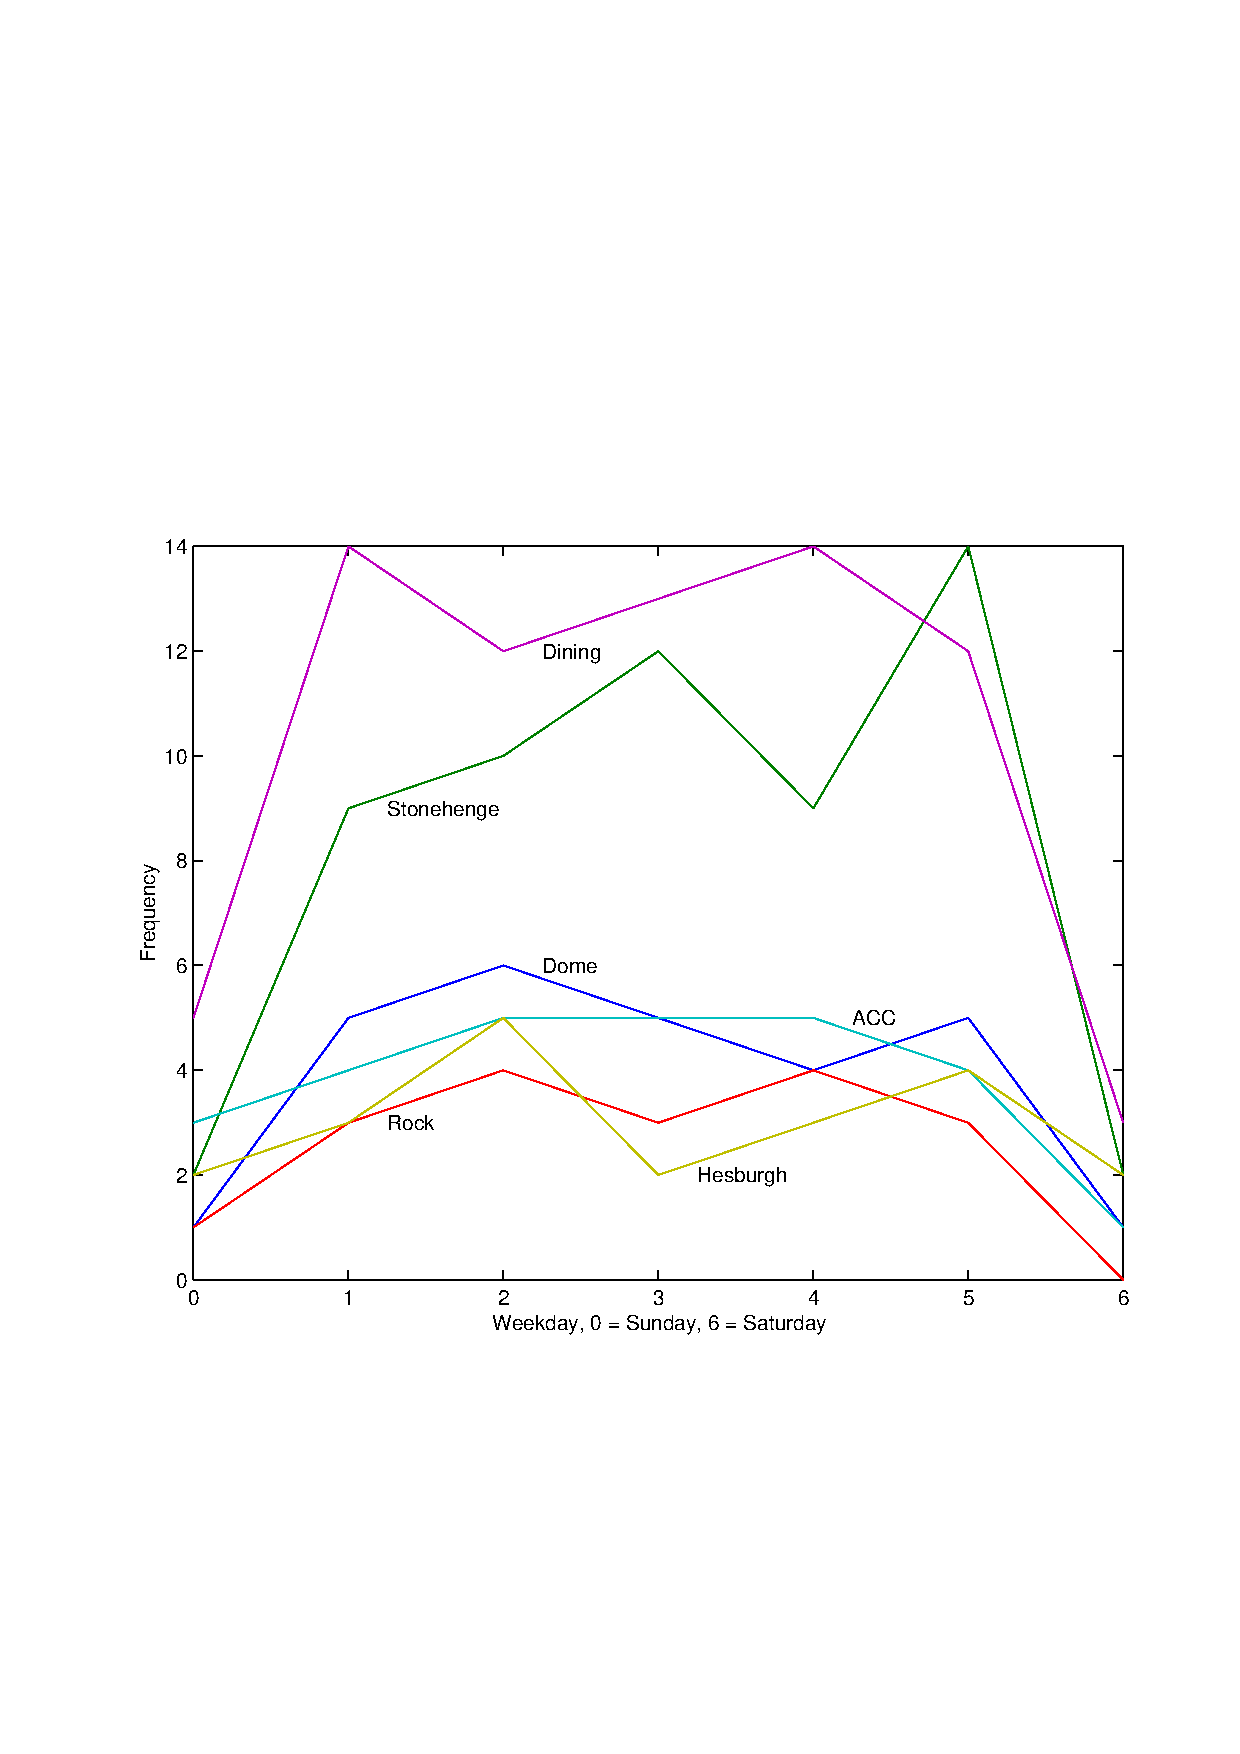
\includegraphics[scale=0.8]{sample_nd}}
    \caption{Location distributions by day of where, where the X axis
      is the weekday (0 through 6), and the Y axis is the sighting
      frequency}
    \label{fig:bogus3}
  \end{center}
\end{figure}

Gnus typically tend to come out when there are large gatherings of
humans with food.  Gnus work very hard at providing us with all the
things that we like (trees, dirt, air, etc.), and so we should freely
give them food.  They will come up and stand a respectful distance
away from you, waiting to see if they will be rewarded for their
efforts.  If you offer some food, they will take it and back off a
respectful distance in order to consume their food while leaving you
to your ``personal space.''  

\section{Groovin' Gnus}
\label{sec:groovin-gnus}

Gnus do tend to stay away from humans in their normal day-to-day
workings.  This is mainly because humans don't, for the most part,
understand what they are doing.  If a Gnu is working, and a human
approaches it, the Gnu will tend to drop whatever it is doing and run
away.  This is probably do to the tendency for humans to have ``group
meetings'' and ``productivity seminars.''  Most Gnus are deathly
afraid of such overmanagement, and run at the slightest hint of it,
for fear that it will cripple their real work.

It is interesting, however, that Gnus have chosen an Institution of
Higher Education for their BOO.\footnote{Base of Operations.}  It is
often said that:
\begin{quote}
  Academic politics are the dirtiest, meanest, ugliest, and generally
  the most low-down, in-your-face, and kick-em-while-they're-down than
  anywhere else (even Washington D.C.)  because the stakes are so low.
\end{quote}
It has been hypothesized that the Gnus are subtly trying to affect a
change for the better (i.e., eliminating the overmanagement problems)
by working the very system that they are trying to change, from
within.  That is, the graduates from Notre Dame can learn from the
examples of the Gnus here, and run screaming (or chattering) at the
slightest hint of overmanagement, and let the real work proceed
unhindered.

% % uncomment the following lines,
% if using chapter-wise bibliography
%
% \bibliographystyle{ndnatbib}
% \bibliography{example}

\chapter{فضاهای فشرده پایدار و فضاهای مرتب فشرده}
\thispagestyle{empty}
\section{فضاهای فشرده پایدار}
یک فضای توپولوژیک جزئاً مرتب (یا به طور خلاصه، فضای مرتب)، از دیدگاه آبرامسکی
\cite{abramsky2}،
مجموعه‌ای مانند $ X $ همراه 
با یک توپولوژی $ \mathcal{O} $ و یک ترتیب $ \leq $ است به طوری که گراف ترتیب در $X\times X  $ بسته باشد. بنابراین ...
\section{فضاهای مرتب فشرده}
در این  بخش به بیان ...
\chapter{اندازه‌ها و ارزیابی‌ها}
\thispagestyle{empty}
\section{اندازه‌ها و تابعی‌های خطی مثبت روی $\mathrm{C(X)}$}
فرض کنید $X$ یک فضای توپولوژیکی روی ...
\section{تابعی‌های خطی}
در این بخش ...
\appendix
\chapter{Test Appendix with a very long title in order to test spacing behavior} \label{app:test}
\lipsum[2]

A convenient form for representing substantial numerical or textual data is a table. 
Table~\ref{tab:test} shows an example of this functionality in \LaTeX.
\begin{table}
  \centering
  \caption{Test table. With an extra-long caption to test spacing functionality for table captions. And inline mathematics.}
  \begin{tabular}{lrr}
    \toprule
    Heading 1 ($u_x$)  & Head 2 & Head 3 \\
    \midrule
    Analytical         & 1.000  & 1.000  \\
    Forward Difference & 0.973  & 0.976  \\
    \bottomrule
  \end{tabular}
  \label{tab:test}
\end{table}
Diagrams, plots, and other graphics should be placed in figures. 
Figure~\ref{fig:test} shows an example of such an environment.
The command \verb+\includegraphics+ from the \verb+graphicx+ package may be used to include external graphics in a wide variety of formats.
\begin{figure}
  \centering 
  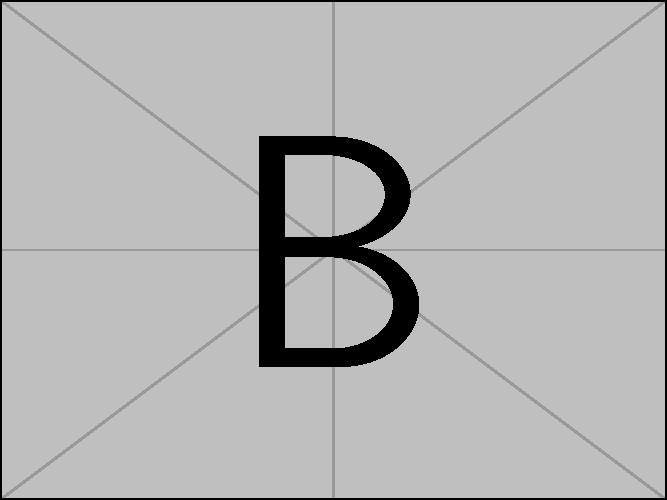
\includegraphics[width=1in]{example-image-b}
  \caption{This test figure tests captions and Table of Contents 
    behavior for lengthy captions.}
  \label{fig:test}
\end{figure}

\section{This is a Very Long Heading to Test the Table of Contents Behavior for Very Long Section Headings}
Sample text. Sample text.

\subsection{This is an Extremely Long Subsection Heading to Test Spacing Behavior for Subsections}
\lipsum[3]

\subsubsection{This is an Extremely Long Subsubsection Heading to Test Spacing Behavior for Subsubsections}
\lipsum[4-5]

% مراجع خود را در این قسمت وارد کنید.
% دستوری برای کوچک کردن اندازه فونت‌ها 
\small
% شروع محیط مراجع 
\begin{thebibliography}{9}
\bibitem{semi}
دامن‌افشان، وحید، \textbf{دامنه توانی احتمالی برای فضاهای فشرده پایدار با استفاده از فضاهای مرتب فشرده}، سمینار کارشناسی ارشد، دانشگاه تبریز، تبریز، ۱۳۸۸.
\begin{LTRitems}
\resetlatinfont

\bibitem{abramsky1}
S. Abramsky, {\em Domain theory in logical form}, Ann. Pure Applied Logic 51 (1991) 1–77.

\bibitem{abramsky2}
S. Abramsky, A. Jung, {\em Domain theory}, in: S. Abramsky, D.M. Gabbay, T.S.E. Maibaum (Eds.), Handbook of
Logic in Computer Science, Vol. 3, Clarendon Press, Oxford, 1994, pp. 1–68.

\bibitem{aliprantis}
C.D. Aliprantis and O. Burkinshaw,   {\em Principles of Real Analysis}.  Academic Press.

\bibitem{alvarez1}
M. Alvarez-Manilla, {\em Measure theoretic results for continuous valuations on partially ordered spaces}, Ph.D.
thesis, Imperial College, University of London, 2001.

\bibitem{alvarez2}
M. Alvarez-Manilla, A. Edalat, N. Saheb-Djahromi, {\em An extension result for continuous valuations}, J. London
Math. Soc. 61 (2000) 629–640.

\bibitem{mainarticle}
M. Alvarez-Manilla, A. Jung, K. Keimel, {\em The probabilistic powerdomain for stably compact
spaces}, Theoretical Computer Science 328 (2004) 221 – 244.

\bibitem{birkhoff}
G. Birkhoff, {\em Lattice Theory}, 3rd Edition, AMS Colloq. Publication, Vol. 25, American Mathematical Society,
Providence, 1967.

\bibitem{choq3}
G. Choquet, {\em Lectures on Analysis}, Vol. 1, W. A. Benjamin Inc., London, 1969.

\bibitem{desh}
J. Desharnais, V. Gupta, R. Jagadeesan, P. Panangaden, {\em Metrics for labeled Markov systems}, in: J.C.M.
Baeten, S. Mauw (Eds.), Proc. 10th Internat. Conf. on Concurrency Theory, Lecture Notes in Computer
Science, Vol. 1664, Springer, Berlin, 1999, pp. 258–273.

\bibitem{edward1}
D.A. Edwards, {\em On the existence of probability measures with given marginals}, Ann. Inst. Fourier, Grenoble,
28 (1978) 53–78.

\bibitem{folland}
G.B. Folland, {\em Real Analysis: Modern Techniques and Their Applications}, 2nd Edition, Wiley, 1999.

\bibitem{gierz1}
G. Gierz, K.H. Hofmann, K. Keimel, J.D. Lawson, M. Mislove, D.S. Scott, {\em A Compendium of Continuous
Lattices}, Springer, Berlin, 1980.

\bibitem{gierz2}
G. Gierz, K.H. Hofmann, K. Keimel, J.D. Lawson, M. Mislove, D.S. Scott, {\em Continuous Lattices and
Domains}, Encyclopedia of Mathematics and its Applications, Vol. 93, Cambridge University Press,
Cambridge, 2003.

\bibitem{horn}
A. Horn, A. Tarski, {\em Measures on Boolean algebras}, Trans. Amer. Math. Soc. 64 (1948) 467–497.

\end{LTRitems}
\end{thebibliography}
\baselineskip=.75cm
\chapter*{واژه‌نامه فارسی به انگلیسی}\markboth{واژه‌نامه فارسی به انگلیسی}{واژه‌نامه فارسی به انگلیسی}
\addcontentsline{toc}{chapter}{واژه‌نامه فارسی به انگلیسی}
\thispagestyle{empty}

\englishgloss{Probabilistic}{احتمالی}
\englishgloss{Valuation}{ارزیابی}
\englishgloss{Measure}{اندازه }
\englishgloss{Stably}{پایدار}
\englishgloss{Weak Topology}{توپولوژی ضعیف}
\englishgloss{Powerdomain}{دامنه‌توانی}
\englishgloss{Function Space}{فضای تابع}
\englishgloss{Semantic Domain}{دامنه معنایی}
\englishgloss{Program Fragment}{قطعه‌برنامه}
\englishgloss{Dcpo}{مجموعه جزئاً مرتب کامل جهت‌دار}
\englishgloss{Ordered}{مرتب}
\chapter*{واژه‌نامه  انگلیسی به  فارسی}\markboth{واژه‌نامه  انگلیسی به  فارسی}{واژه‌نامه  انگلیسی به  فارسی}
\addcontentsline{toc}{chapter}{واژه‌نامه  انگلیسی به  فارسی}
\thispagestyle{empty}

\persiangloss{مجموعه جزئاً مرتب کامل جهت‌دار}{Dcpo}
\persiangloss{فضای تابع}{Function Space}
\persiangloss{اندازه }{Measure}
\persiangloss{مرتب}{Ordered}
\persiangloss{دامنه‌توانی}{Powerdomain}
\persiangloss{احتمالی}{Probabilistic}
\persiangloss{قطعه‌برنامه}{Program Fragment}
\persiangloss{دامنه معنایی}{Semantic Domain}
\persiangloss{پایدار}{Stably}
\persiangloss{ارزیابی}{Valuation}
\persiangloss{توپولوژی ضعیف}{Weak Topology}

\printindex
% در این فایل، عنوان پایان‌نامه، مشخصات خود و چکیده پایان‌نامه را به انگلیسی، وارد کنید.
% توجه داشته باشید که جدول حاوی مشخصات پروژه/پایان‌نامه/رساله، به طور خودکار، رسم می‌شود.
%%%%%%%%%%%%%%%%%%%%%%%%%%%%%%%%%%%%
\baselineskip=.6cm
\begin{latin}
\latinuniversity{University of Tabriz}
\latinfaculty{Faculty Of Mathematical Sciences}
\latinsubject{Pure Mathematics}
\latinfield{Mathematical Analysis}
\latintitle{Writing Projects, Theses, and Dissertations Using \textsf{tabriz-thesis} Class}
\firstlatinsupervisor{First Supervisor}
%\secondlatinsupervisor{Second Supervisor}
\firstlatinadvisor{First Advisor}
%\secondlatinadvisor{Second Advisor}
\latinname{Vahid}
\latinsurname{Damanafshan}
\latinthesisdate{2011}
\latinkeywords{Probabilistic powerdomain; Stably compact space; Valuation}
\en-abstract{
This thesis studies on writing projects, theses and dissertations using \textsf{tabriz-thesis} Class. It ...
}
\latinvtitle
\end{latin}

\label{LastPage}
\end{document}